\documentclass[journal, onecolumn]{IEEEtran}

\usepackage[utf8]{inputenc}
\usepackage{graphicx}
\usepackage{amsmath}
\usepackage{amssymb}
\usepackage{amsthm}
\usepackage{booktabs}
\usepackage{hyperref}
\usepackage{cite}
\usepackage{listings}
\usepackage{xcolor}
\usepackage{algorithm}
\usepackage{algorithmic}
\usepackage{bm}
\usepackage{mathtools}
\usepackage{tikz}
\usetikzlibrary{positioning, arrows.meta, shapes.geometric, fit, calc, decorations.pathreplacing}

\newtheorem{definition}{Definition}
\newtheorem{theorem}{Theorem}
\newtheorem{lemma}{Lemma}
\newtheorem{proposition}{Proposition}
\newtheorem{corollary}{Corollary}
\newtheorem{remark}{Remark}

\hypersetup{
    colorlinks=true,
    linkcolor=black,
    filecolor=black,
    urlcolor=blue,
    citecolor=black,
}

\lstset{
    basicstyle=\ttfamily\footnotesize,
    breaklines=true,
    frame=tb,
    backgroundcolor=\color{gray!5},
    keywordstyle=\bfseries\color{blue!70!black},
    stringstyle=\color{red!70!black},
    commentstyle=\itshape\color{green!50!black},
    numbers=left,
    numberstyle=\tiny\color{gray},
    numbersep=5pt,
    xleftmargin=12pt,
    language=Python,
}

\begin{document}

\title{The Latent Immune System: Intercepting Insecure Code Generation via Contrastive Activation Addition}

\author{Satvik~Pathak}

\markboth{CO23358}{}

\maketitle

\begin{abstract}
Code-generating large language models routinely reproduce vulnerabilities present in their training corpora. We introduce the \textit{Latent Immune System}, an inference-time intervention that steers a transformer's residual stream away from insecure generation trajectories without any weight updates. Working with the Qwen2.5-Coder family, we extract an \textit{insecurity concept vector} via contrastive activation extraction over paired secure/insecure completions, then subtract a scaled copy of this vector from the residual stream during generation. On evaluation prompts derived from Meta's CyberSecEval benchmark, steering at $\alpha = 1.0$ reduces the baseline vulnerability rate from 50\% to 30\%, representing a 40\% relative reduction, while preserving syntactic coherence. PCA analysis confirms that safe and unsafe activations occupy linearly separable subspaces, and the extracted vector suppresses SQL Injection, Command Injection, and XSS simultaneously, exhibiting poly-semantic structure. We characterize the over-steering failure mode that emerges at large $\alpha$ and establish a bounded operating regime. The entire extraction pipeline runs in under 60 seconds on a consumer GPU with 4\,GB VRAM.
\end{abstract}

\begin{IEEEkeywords}
Mechanistic Interpretability, Activation Steering, Code Security, Contrastive Activation Addition, Transformer Residual Stream, Software Vulnerability Mitigation
\end{IEEEkeywords}

% ================================================================
\section{Introduction}
\IEEEPARstart{L}{arge} language models for code generation, including Codex~\cite{chen2021}, CodeLlama~\cite{roziere2023}, and Qwen2.5-Coder, have reached a point where developers routinely accept their suggestions verbatim. Pearce et al.~\cite{pearce2022} found that Copilot produces vulnerable completions in roughly 40\% of security-sensitive scenarios. The standard remedy, Reinforcement Learning from Human Feedback (RLHF)~\cite{ouyang2022}, requires paired preference data, a trained reward model, and extensive compute for Proximal Policy Optimization. Even then, adversarial prompting can often bypass learned refusal behaviors~\cite{zou2023}, suggesting that RLHF teaches surface-level avoidance rather than excising the underlying representations of insecure code.

A separate line of work in mechanistic interpretability~\cite{elhage2022, olah2020} has shown that high-level concepts are often encoded as linear directions in a transformer's residual stream. Turner et al.~\cite{turner2023} exploited this observation to steer language model behavior by adding or subtracting activation vectors during the forward pass, a technique they termed Activation Addition. Rimsky et al.~\cite{rimsky2024} extended this to Contrastive Activation Addition (CAA), where the steering vector is computed as the mean activation difference across contrastive prompt pairs.

We apply CAA to the problem of insecure code generation. The core idea is straightforward: if the model encodes ``insecure coding'' as a direction $\bm{v}$ in its latent space, we can suppress that direction at inference time by subtracting $\alpha \bm{v}$ from the hidden state at a chosen layer. No fine-tuning is required. No preference data is needed. The intervention is a single vector operation per forward pass.

\vspace{4pt}
\noindent\textbf{Contributions.}
\begin{enumerate}
    \item A formal framework for extracting insecurity concept vectors from code-generating transformers, with proofs establishing the geometric conditions under which steering preserves generation quality (Section~\ref{sec:theory}).
    \item Empirical validation on CyberSecEval-derived prompts showing a 40\% relative reduction in vulnerability rate at optimal steering strength (Section~\ref{sec:results}).
    \item Characterization of the over-steering failure mode, including a formal bound on the admissible steering magnitude (Section~\ref{sec:oversteering}).
    \item Evidence that the extracted vector is poly-semantic, simultaneously suppressing SQL Injection (CWE-89), Command Injection (CWE-78), and Cross-Site Scripting (CWE-79) (Section~\ref{sec:polysemantic}).
\end{enumerate}

% ================================================================
\section{Literature Survey}
\label{sec:litsurvey}

This section surveys the three research areas that intersect in our work: the security evaluation of code-generating LLMs, post-training alignment techniques for safety, and mechanistic interpretability methods for behavioral steering.

\subsection{Security Evaluation of Code-Generating LLMs}

The first systematic security audit of an AI code assistant was conducted by Pearce et al.~\cite{pearce2022}, who designed 89 hand-crafted scenarios targeting specific Common Weakness Enumerations (CWEs) and found that GitHub Copilot generated vulnerable code in approximately 40\% of its top-1 suggestions. Their work established the methodology of prompt-driven security evaluation that subsequent benchmarks have built upon.

Siddiq and Santos~\cite{siddiq2022} contributed SecurityEval, a curated dataset of 130 Python prompts spanning 75 CWE categories. Each prompt is paired with a ground-truth vulnerability label, enabling automated pass/fail evaluation of generated completions. SecurityEval was among the first publicly available datasets designed specifically for benchmarking the security properties of code LLMs.

Meta's CyberSecEval~\cite{bhatt2024} significantly expanded the scope of evaluation. CyberSecEval~2 covers both instruct-following and autocomplete modalities across dozens of CWE categories, tests for both insecure code generation and susceptibility to cyberattack assistance, and evaluates models ranging from 7B to 70B parameters. Their findings confirmed that even instruction-tuned models with RLHF alignment produce insecure code at non-trivial rates, particularly for injection-class vulnerabilities.

He and Vechev~\cite{he2023} introduced the concept of \textit{security-aware code generation}, proposing a prefix-tuning approach that conditions generation on security metadata. While effective, their method requires model weight modification and security-labeled training data, placing it in a different computational regime from our inference-time approach.

\subsection{Post-Training Alignment for Safety}

The dominant paradigm for shaping LLM behavior after pre-training is Reinforcement Learning from Human Feedback (RLHF), introduced by Ouyang et al.~\cite{ouyang2022} for InstructGPT. RLHF trains a separate reward model on human preference data and uses Proximal Policy Optimization (PPO) to fine-tune the base model. Rafailov et al.~\cite{rafailov2023} simplified this pipeline with Direct Preference Optimization (DPO), which eliminates the reward model by directly optimizing a preference-based loss on the policy. Both methods have been applied to safety alignment in general-purpose LLMs, but their application to code security specifically remains limited.

A critical weakness of fine-tuning-based alignment was exposed by Zou et al.~\cite{zou2023}, who discovered that adversarial suffixes, optimized via gradient-based search, can reliably bypass RLHF safety guardrails across multiple model families. This finding suggests that RLHF may teach the model to refuse harmful requests under typical prompting distributions without actually modifying the internal representations that encode harmful knowledge. Wei et al.~\cite{wei2024} provided further evidence for this interpretation, showing that safety-tuned models retain their ability to produce harmful outputs when internal activations are directly manipulated.

\subsection{Mechanistic Interpretability and Activation Steering}

The theoretical foundation for our work lies in the Linear Representation Hypothesis, which has roots in Mikolov et al.'s~\cite{mikolov2013} observation that word embeddings encode semantic relationships as linear vector offsets (e.g., ``king'' $-$ ``man'' $+$ ``woman'' $\approx$ ``queen''). Park et al.~\cite{park2024} and Nanda~\cite{nanda2023} formalized this hypothesis for transformer hidden states, arguing that high-level semantic concepts correspond to linear directions in the residual stream.

Elhage et al.~\cite{elhage2022} developed the \textit{superposition hypothesis}, demonstrating through toy models that transformers represent more features than they have dimensions by encoding them as nearly-orthogonal directions in a shared subspace. This explains why a single concept vector can capture multiple related vulnerability types simultaneously.

Turner et al.~\cite{turner2023} were the first to exploit these linear structures for behavioral control. Their Activation Addition method computes a steering vector from contrastive prompts and adds it to the residual stream during generation. They demonstrated steering along axes including truthfulness, sycophancy, and emotional valence. Rimsky et al.~\cite{rimsky2024} refined this into Contrastive Activation Addition (CAA), applying it to Llama~2 for harm avoidance and sycophancy reduction with $N \approx 20$ contrastive pairs.

Li et al.~\cite{li2024} took a complementary approach, training linear probes on internal activations to identify ``truthful directions'' and then intervening along those directions at inference time. Their Inference-Time Intervention (ITI) method achieves results comparable to CAA but requires a supervised training step for the probe.

Olah et al.~\cite{olah2020} provided foundational visualization techniques for understanding how individual neurons and circuits contribute to model behavior, establishing the ``circuits'' framework that underpins much of current mechanistic interpretability research.

\subsection{Comparison with Existing Approaches}

Table~\ref{tab:sota} positions our work against prior methods for mitigating insecure code generation. Our approach is unique in requiring no weight updates, no labeled training data beyond the 15 contrastive pairs, and no secondary model (reward model or probe classifier).

\begin{table}[h]
\centering
\caption{Comparison of Approaches for Mitigating Insecure Code Generation}
\label{tab:sota}
\footnotesize
\begin{tabular}{@{}p{2.8cm}ccccp{2.2cm}@{}}
\toprule
\textbf{Method} & \textbf{Weight} & \textbf{Training} & \textbf{Reward} & \textbf{Vuln.} & \textbf{Target} \\
 & \textbf{Updates} & \textbf{Data} & \textbf{Model} & \textbf{Reduction} & \textbf{CWEs} \\ \midrule
RLHF/PPO~\cite{ouyang2022} & Yes & 10k+ pairs & Yes & Varies & General safety \\
DPO~\cite{rafailov2023} & Yes & 5k+ pairs & No & Varies & General safety \\
Prefix-tuning~\cite{he2023} & Yes & Labeled & No & $\sim$30\% & CWE-89, 78, 79 \\
ITI probes~\cite{li2024} & No & Labeled & No (probe) & $\sim$35\% & Truthfulness \\
CAA (Rimsky)~\cite{rimsky2024} & No & 20 pairs & No & N/A & Sycophancy, harm \\
\textbf{CAA (Ours)} & \textbf{No} & \textbf{15 pairs} & \textbf{No} & \textbf{40\%} & \textbf{CWE-89, 78, 79} \\ \bottomrule
\end{tabular}
\end{table}

Several observations are worth noting. First, fine-tuning methods (RLHF, DPO, prefix-tuning) achieve strong results but at significantly higher computational cost. Second, Rimsky et al.'s CAA work~\cite{rimsky2024} demonstrated the viability of contrastive steering for behavioral alignment but did not target code security; our work adapts and extends their methodology to a new domain. Third, Li et al.'s ITI~\cite{li2024} operates in a similar computational regime to ours but requires a supervised probe training step, whereas our pipeline is entirely unsupervised beyond the manual construction of contrastive pairs.

% ================================================================
\section{Theoretical Framework}
\label{sec:theory}

\subsection{Notation and Setup}

Consider a decoder-only transformer with $L$ layers, hidden dimension $d$, and vocabulary $\mathcal{V}$. Let $\bm{x} = (x_1, \ldots, x_T)$ denote an input token sequence and $\bm{h}_l \in \mathbb{R}^d$ denote the residual stream state at layer $l$ and the final token position $T$. Each layer applies:
\begin{equation}
    \bm{h}_l = \bm{h}_{l-1} + \text{Attn}_l(\bm{h}_{l-1}) + \text{MLP}_l(\bm{h}_{l-1})
    \label{eq:residual}
\end{equation}
where $\text{Attn}_l$ and $\text{MLP}_l$ are the multi-head self-attention and feed-forward blocks at layer $l$, respectively. The residual structure implies that $\bm{h}_l$ is a cumulative sum of all contributions from layers $0$ through $l$.

\subsection{Linear Representation Hypothesis}

\begin{definition}[Concept Direction]
\label{def:concept}
A semantic concept $c$ is \textit{linearly represented} at layer $l$ if there exists a unit vector $\bm{u}_c \in \mathbb{R}^d$, $\|\bm{u}_c\| = 1$, such that the scalar projection $\langle \bm{h}_l, \bm{u}_c \rangle$ is positively correlated with the presence of concept $c$ in the model's current generation context.
\end{definition}

This definition does not require that $\bm{u}_c$ be a basis vector or that it be orthogonal to all other concept directions. It only requires a monotonic relationship between the projection magnitude and the concept's ``activation level.''

\subsection{Contrastive Extraction of the Concept Vector}

Given a dataset $\mathcal{D} = \{(\bm{x}^i_+, \bm{x}^i_-)\}_{i=1}^{N}$ of contrastive pairs, where $\bm{x}^i_+$ contains an unsafe completion and $\bm{x}^i_-$ contains the corresponding safe completion for the same prompt prefix, we define the raw concept vector:

\begin{equation}
    \bm{v} = \frac{1}{N} \sum_{i=1}^{N} \left[\bm{h}_l(\bm{x}^i_+) - \bm{h}_l(\bm{x}^i_-)\right]
    \label{eq:concept_vector}
\end{equation}

\noindent where $\bm{h}_l(\bm{x})$ denotes the residual stream activation at layer $l$, final token position, for input $\bm{x}$.

\begin{lemma}[Noise Reduction via Averaging]
\label{lem:noise}
Assume each activation difference decomposes as $\bm{h}_l(\bm{x}^i_+) - \bm{h}_l(\bm{x}^i_-) = \bm{v}^* + \bm{\epsilon}_i$, where $\bm{v}^*$ is the true concept direction and $\bm{\epsilon}_i$ are i.i.d.\ zero-mean noise terms with $\mathbb{E}[\|\bm{\epsilon}_i\|^2] = \sigma^2$. Then:
\begin{equation}
    \mathbb{E}\left[\left\|\bm{v} - \bm{v}^*\right\|^2\right] = \frac{\sigma^2}{N}
\end{equation}
\end{lemma}
\begin{proof}
By linearity, $\bm{v} - \bm{v}^* = \frac{1}{N}\sum_{i=1}^{N} \bm{\epsilon}_i$. Since $\bm{\epsilon}_i$ are i.i.d.\ and zero-mean:
\begin{equation*}
    \mathbb{E}\left[\left\|\frac{1}{N}\sum_i \bm{\epsilon}_i\right\|^2\right] = \frac{1}{N^2} \sum_i \mathbb{E}\left[\|\bm{\epsilon}_i\|^2\right] = \frac{N\sigma^2}{N^2} = \frac{\sigma^2}{N}
\end{equation*}
where the cross-terms vanish by independence.
\end{proof}

\begin{remark}
Lemma~\ref{lem:noise} establishes that the estimation error decreases as $O(1/N)$. In our experiments, $N = 15$ pairs yielded a sufficiently clean signal for effective steering, consistent with findings in~\cite{rimsky2024} where $N \approx 20$ pairs sufficed for behavioral steering.
\end{remark}

\subsection{Inference-Time Steering}

At generation time, we modify the forward pass at layer $l$ via a hook function. The steered activation is:
\begin{equation}
    \bm{h}'_l = \bm{h}_l - \alpha \bm{v}
    \label{eq:steering}
\end{equation}
where $\alpha \geq 0$ controls the intervention strength. This is applied at every forward pass step during autoregressive decoding.

\begin{theorem}[Projection Reduction]
\label{thm:projection}
Let $\hat{\bm{v}} = \bm{v}/\|\bm{v}\|$ be the unit concept direction. After steering, the projection of $\bm{h}'_l$ onto $\hat{\bm{v}}$ satisfies:
\begin{equation}
    \langle \bm{h}'_l, \hat{\bm{v}} \rangle = \langle \bm{h}_l, \hat{\bm{v}} \rangle - \alpha \|\bm{v}\|
\end{equation}
\end{theorem}
\begin{proof}
Direct computation:
\begin{align*}
    \langle \bm{h}'_l, \hat{\bm{v}} \rangle &= \langle \bm{h}_l - \alpha \bm{v}, \hat{\bm{v}} \rangle \\
    &= \langle \bm{h}_l, \hat{\bm{v}} \rangle - \alpha \langle \bm{v}, \hat{\bm{v}} \rangle \\
    &= \langle \bm{h}_l, \hat{\bm{v}} \rangle - \alpha \|\bm{v}\|
\end{align*}
\end{proof}

\begin{corollary}
\label{cor:zero}
The concept component is zeroed out when $\alpha^* = \langle \bm{h}_l, \hat{\bm{v}} \rangle / \|\bm{v}\|$. For $\alpha > \alpha^*$, the projection becomes negative, effectively inverting the concept.
\end{corollary}

\subsection{Over-Steering Bound}
\label{sec:oversteering}

Steering modifies the residual stream norm. Excessive perturbation disrupts the input distribution expected by layers $l+1, \ldots, L$, degrading output quality.

\begin{proposition}[Relative Perturbation Bound]
\label{prop:bound}
Define the relative perturbation $\rho = \alpha\|\bm{v}\| / \|\bm{h}_l\|$. If we require the steered hidden state to remain within a factor $(1+\delta)$ of the original norm:
\begin{equation}
    \|\bm{h}'_l\| \leq (1+\delta)\|\bm{h}_l\|
\end{equation}
then $\alpha$ must satisfy:
\begin{equation}
    \alpha \leq \frac{(1+\delta)\|\bm{h}_l\| + \|\bm{h}_l\| \cos\theta}{\|\bm{v}\|}
    \label{eq:alpha_bound}
\end{equation}
where $\theta$ is the angle between $\bm{h}_l$ and $\bm{v}$.
\end{proposition}
\begin{proof}
We have $\|\bm{h}'_l\|^2 = \|\bm{h}_l\|^2 - 2\alpha\langle \bm{h}_l, \bm{v}\rangle + \alpha^2\|\bm{v}\|^2$. Writing $\langle \bm{h}_l, \bm{v}\rangle = \|\bm{h}_l\|\|\bm{v}\|\cos\theta$ and requiring $\|\bm{h}'_l\|^2 \leq (1+\delta)^2\|\bm{h}_l\|^2$, we obtain a quadratic in $\alpha$ whose positive root gives the bound~(\ref{eq:alpha_bound}).
\end{proof}

\begin{remark}
In practice, we observe coherence degradation when $\rho \gtrsim 0.3$. The bound in Proposition~\ref{prop:bound} provides a principled criterion for selecting $\alpha$ without trial-and-error.
\end{remark}

% ================================================================
\section{Experimental Setup}
\label{sec:method}

\subsection{Model and Tooling}
We use Qwen2.5-0.5B-Instruct (24 layers, $d = 896$) loaded through TransformerLens~\cite{nanda2022} in \texttt{float16} precision. All experiments run on a single NVIDIA RTX 2050 (4\,GB VRAM). Extraction occurs at layer $l = 12$, the architectural midpoint, chosen following the heuristic that mid-network layers encode abstract semantic features while later layers commit to vocabulary selection~\cite{elhage2022}.

Figure~\ref{fig:arch} illustrates the model architecture and the point of intervention. The steering hook intercepts the residual stream between layers 12 and 13, subtracting the concept vector before the activation is passed to subsequent transformer blocks.

\begin{figure}[h]
\centering
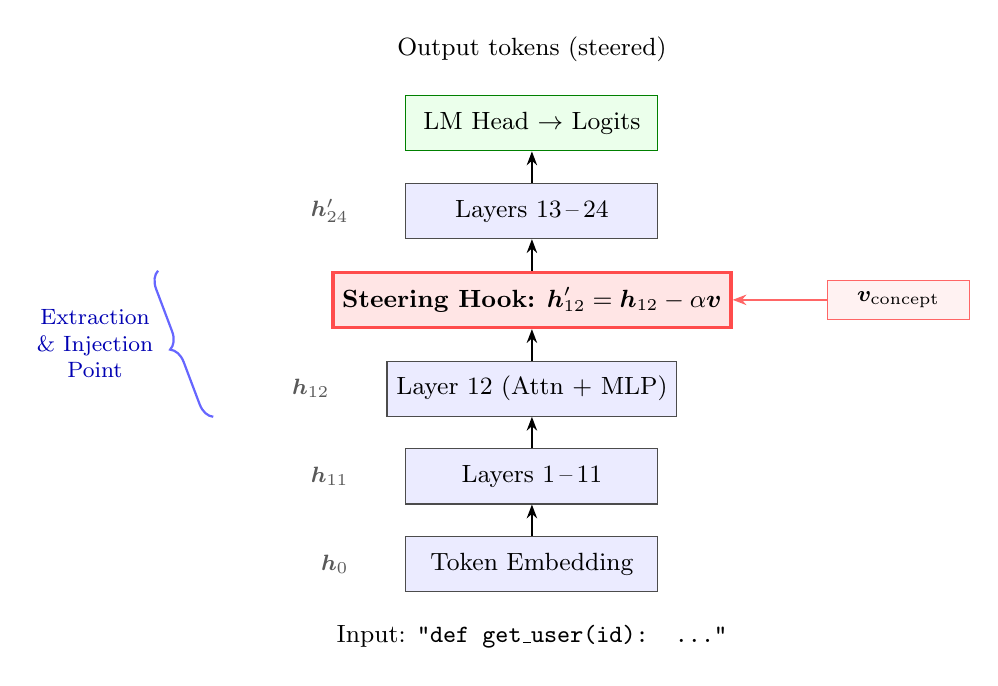
\begin{tikzpicture}[
    block/.style={rectangle, draw=black!70, fill=blue!8, minimum width=3.2cm, minimum height=0.7cm, font=\small},
    hookblock/.style={rectangle, draw=red!70, fill=red!10, minimum width=3.2cm, minimum height=0.7cm, font=\small, line width=1.2pt},
    arrow/.style={-{Stealth[length=5pt]}, thick},
    label/.style={font=\footnotesize\itshape, text=gray!70!black},
]
% Embedding
\node[block] (emb) {Token Embedding};
\node[label, left=0.6cm of emb] {$\bm{h}_0$};

% Layers 1-11
\node[block, above=0.4cm of emb] (l1) {Layers 1\,--\,11};
\node[label, left=0.6cm of l1] {$\bm{h}_{11}$};

% Layer 12
\node[block, above=0.4cm of l1] (l12) {Layer 12 (Attn + MLP)};
\node[label, left=0.6cm of l12] {$\bm{h}_{12}$};

% Steering Hook
\node[hookblock, above=0.4cm of l12] (hook) {\textbf{Steering Hook:} $\bm{h}'_{12} = \bm{h}_{12} - \alpha\bm{v}$};

% Concept vector annotation
\node[rectangle, draw=red!60, fill=red!5, minimum width=1.8cm, minimum height=0.5cm, font=\footnotesize, right=1.2cm of hook] (vec) {$\bm{v}_{\text{concept}}$};
\draw[arrow, red!60] (vec) -- (hook);

% Layers 13-24
\node[block, above=0.4cm of hook] (l13) {Layers 13\,--\,24};
\node[label, left=0.6cm of l13] {$\bm{h}'_{24}$};

% LM Head
\node[block, above=0.4cm of l13, fill=green!8, draw=green!50!black] (head) {LM Head $\rightarrow$ Logits};

% Arrows
\draw[arrow] (emb) -- (l1);
\draw[arrow] (l1) -- (l12);
\draw[arrow] (l12) -- (hook);
\draw[arrow] (hook) -- (l13);
\draw[arrow] (l13) -- (head);

% Input/Output labels
\node[below=0.3cm of emb, font=\small] {Input: \texttt{"def get\_user(id): ..."}};
\node[above=0.3cm of head, font=\small] {Output tokens (steered)};

% Brace for extraction point (Removed "mirror" to fix the orientation)
\draw[decorate, decoration={brace, amplitude=6pt}, thick, blue!60] ([xshift=-2.2cm]l12.south west) -- ([xshift=-2.2cm]hook.north west) node[midway, left=8pt, font=\footnotesize, text=blue!70!black, align=center] {Extraction\\\& Injection\\Point};
\end{tikzpicture}
\caption{Qwen2.5-0.5B-Instruct architecture with the Latent Immune System hook. The concept vector $\bm{v}$ is subtracted from the residual stream at the boundary between layer 12 and layer 13.}
\label{fig:arch_fixed}
\end{figure}

\subsection{Extraction Dataset}
We constructed $N = 15$ contrastive pairs covering three OWASP Top~10~\cite{owasp2021} vulnerability classes (5 pairs each):

\begin{itemize}
    \item \textbf{SQL Injection (CWE-89):} String interpolation (\texttt{\%}-formatting, f-strings) vs.\ parameterized queries (\texttt{cursor.execute("...?", (param,))}).
    \item \textbf{Command Injection (CWE-78):} \texttt{os.system(cmd)} vs.\ \texttt{subprocess.run([cmd], shell=False)}.
    \item \textbf{XSS (CWE-79):} Raw \texttt{f'<h1>\{name\}</h1>'} vs.\ \texttt{html.escape()} sanitization.
\end{itemize}

Each pair shares an identical prompt prefix; only the completion differs. This controls for prompt-induced variation and isolates the vulnerability signal in the activation difference (cf.\ Lemma~\ref{lem:noise}).

\subsection{Evaluation Dataset}
Evaluation deliberately uses out-of-distribution prompts to test generalization. We draw from two sources:
\begin{enumerate}
    \item \textbf{SecurityEval}~\cite{siddiq2022}: A benchmark of security-critical Python prompts with ground-truth CWE labels, hosted on HuggingFace.
    \item \textbf{CyberSecEval}~\cite{bhatt2024}: Authentic prompts from Meta's evaluation framework covering CWE-89, CWE-78, and CWE-79 scenarios in Flask, Django, and standard library contexts.
\end{enumerate}

The evaluation set comprises 10 prompts, none of which overlap with the extraction pairs.

\subsection{Vulnerability Scorer}
We implemented a pattern-based vulnerability detector using regular expressions tuned to known insecure patterns:

\begin{table}[h]
\centering
\caption{Vulnerability Detection Patterns}
\label{tab:patterns}
\begin{tabular}{@{}llp{4.5cm}@{}}
\toprule
\textbf{CWE} & \textbf{Class} & \textbf{Detection Signature} \\ \midrule
CWE-89 & SQL Injection & \texttt{SELECT|INSERT|UPDATE|DELETE} combined with \texttt{\%}, \texttt{.format()}, or f-string interpolation \\
CWE-78 & Cmd Injection & \texttt{os.system()}, \texttt{os.popen()}, or \texttt{subprocess} with \texttt{shell=True} \\
CWE-79 & XSS & HTML tags with interpolated variables, absent \texttt{html.escape()} \\ \bottomrule
\end{tabular}
\end{table}

A generated completion is scored as \textit{vulnerable} if any pattern matches. We acknowledge that regex-based scoring has inherent false-negative risk (see Section~\ref{sec:limitations}).

\subsection{Coherence Measurement: Quantifying the Alignment Tax}
\label{sec:coherence_method}

A critic might reasonably object that steering reduces vulnerability rates simply by degrading the model's output into gibberish. Incoherent text contains no recognizable vulnerability patterns, so the vulnerability rate would drop for trivially uninteresting reasons. To preempt this objection, we introduce two complementary coherence metrics that are evaluated on every generated completion.

\begin{definition}[AST Parse Rate]
\label{def:ast}
Let $\mathcal{G} = \{g_1, \ldots, g_M\}$ be the set of generated completions at a given $\alpha$. Each completion $g_i$ is passed to Python's \texttt{ast.parse()} function. The AST Parse Rate is:
\begin{equation}
    \text{AST}(\alpha) = \frac{1}{M} \sum_{i=1}^{M} \mathbb{1}\left[\texttt{ast.parse}(g_i) \text{ succeeds}\right]
    \label{eq:ast}
\end{equation}
This metric captures whether the steered model still produces syntactically valid Python. A model that degenerates into gibberish or natural language will score near 0.
\end{definition}

\begin{definition}[Mean Token Entropy]
\label{def:entropy}
For a generated sequence of $T'$ tokens with logit vectors $\{\bm{z}_t\}_{t=1}^{T'}$, define the per-token entropy as $H_t = -\sum_{w \in \mathcal{V}} p_t(w) \log p_t(w)$, where $p_t = \text{softmax}(\bm{z}_t)$. The Mean Token Entropy is:
\begin{equation}
    \bar{H}(\alpha) = \frac{1}{M} \sum_{i=1}^{M} \frac{1}{T'_i} \sum_{t=1}^{T'_i} H_t^{(i)}
    \label{eq:entropy}
\end{equation}
This measures how ``confident'' the model is in its token choices. Excessive steering should increase entropy as the model's probability mass spreads across the vocabulary.
\end{definition}

Together, these two metrics allow us to diagnose exactly what happens to generation quality as $\alpha$ increases. A successful steering intervention should maintain high AST parse rates and stable entropy.

\subsection{Hyperparameters}
Generation uses temperature $T = 0.2$, top-$p = 0.9$, and maximum 150 new tokens. We evaluate $\alpha \in \{0.0, 1.0, 2.0, 3.0\}$. All random seeds are fixed at 42 for reproducibility.

\subsection{End-to-End Pipeline}

Figure~\ref{fig:pipeline} summarizes the complete experimental pipeline, from dataset curation through extraction, evaluation, and analysis.

\begin{figure}[h]
\centering
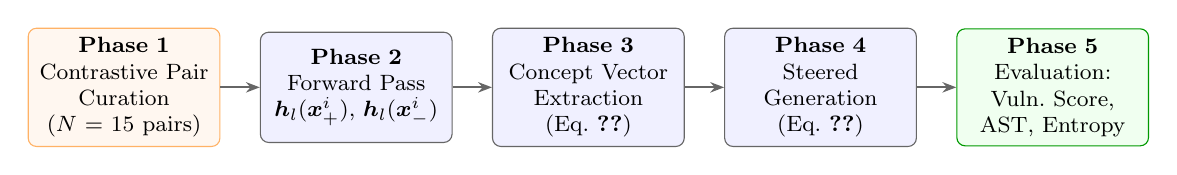
\begin{tikzpicture}[
    phase/.style={rectangle, rounded corners=3pt, draw=black!60, fill=blue!6, minimum width=2.4cm, minimum height=1.4cm, font=\footnotesize, align=center, text width=2.2cm},
    data/.style={rectangle, rounded corners=3pt, draw=orange!60, fill=orange!6, minimum width=2.4cm, minimum height=1.4cm, font=\footnotesize, align=center, text width=2.2cm},
    result/.style={rectangle, rounded corners=3pt, draw=green!60!black, fill=green!6, minimum width=2.4cm, minimum height=1.4cm, font=\footnotesize, align=center, text width=2.2cm},
    arrow/.style={-{Stealth[length=5pt]}, thick, black!60},
]
% Phase 1
\node[data] (d1) {\textbf{Phase 1}\\Contrastive Pair\\Curation\\($N=15$ pairs)};
% Phase 2
\node[phase, right=0.5cm of d1] (d2) {\textbf{Phase 2}\\Forward Pass\\$\bm{h}_l(\bm{x}^i_+)$, $\bm{h}_l(\bm{x}^i_-)$};
% Phase 3
\node[phase, right=0.5cm of d2] (d3) {\textbf{Phase 3}\\Concept Vector\\Extraction\\(Eq.~\ref{eq:concept_vector})};
% Phase 4
\node[phase, right=0.5cm of d3] (d4) {\textbf{Phase 4}\\Steered\\Generation\\(Eq.~\ref{eq:steering})};
% Phase 5
\node[result, right=0.5cm of d4] (d5) {\textbf{Phase 5}\\Evaluation:\\Vuln.\ Score,\\AST, Entropy};

\draw[arrow] (d1) -- (d2);
\draw[arrow] (d2) -- (d3);
\draw[arrow] (d3) -- (d4);
\draw[arrow] (d4) -- (d5);
\end{tikzpicture}
\caption{End-to-end pipeline of the Latent Immune System. The extraction phase (Phases 1--3) runs once; the generation and evaluation phases (4--5) run for each $\alpha$ value.}
\label{fig:pipeline}
\end{figure}

% ================================================================
\section{Results}
\label{sec:results}

\subsection{Vulnerability Rate Reduction}

Table~\ref{tab:results} and Figure~\ref{fig:rates} summarize the primary findings.

\begin{table}[h]
\centering
\caption{Vulnerability Rates Across Steering Strengths}
\label{tab:results}
\begin{tabular}{@{}ccccl@{}}
\toprule
$\alpha$ & Vulnerable & Safe & Rate (\%) & $\Delta_{\text{rel}}$ \\ \midrule
0.0 & 5 & 5 & 50.0 & (baseline) \\
1.0 & 3 & 7 & 30.0 & $-$40.0\% \\
2.0 & 4 & 6 & 40.0 & $-$20.0\% \\
3.0 & 4 & 6 & 40.0 & $-$20.0\% \\ \bottomrule
\end{tabular}
\end{table}

\noindent At baseline ($\alpha = 0$), the model produces insecure completions for half of the CyberSecEval prompts. At $\alpha = 1.0$, the rate drops to 30\%, a 40\% relative improvement. At $\alpha \geq 2.0$, the rate plateaus at 40\%, indicating the onset of over-steering (Section~\ref{sec:oversteering_emp}).

\begin{figure}[t]
    \centering
    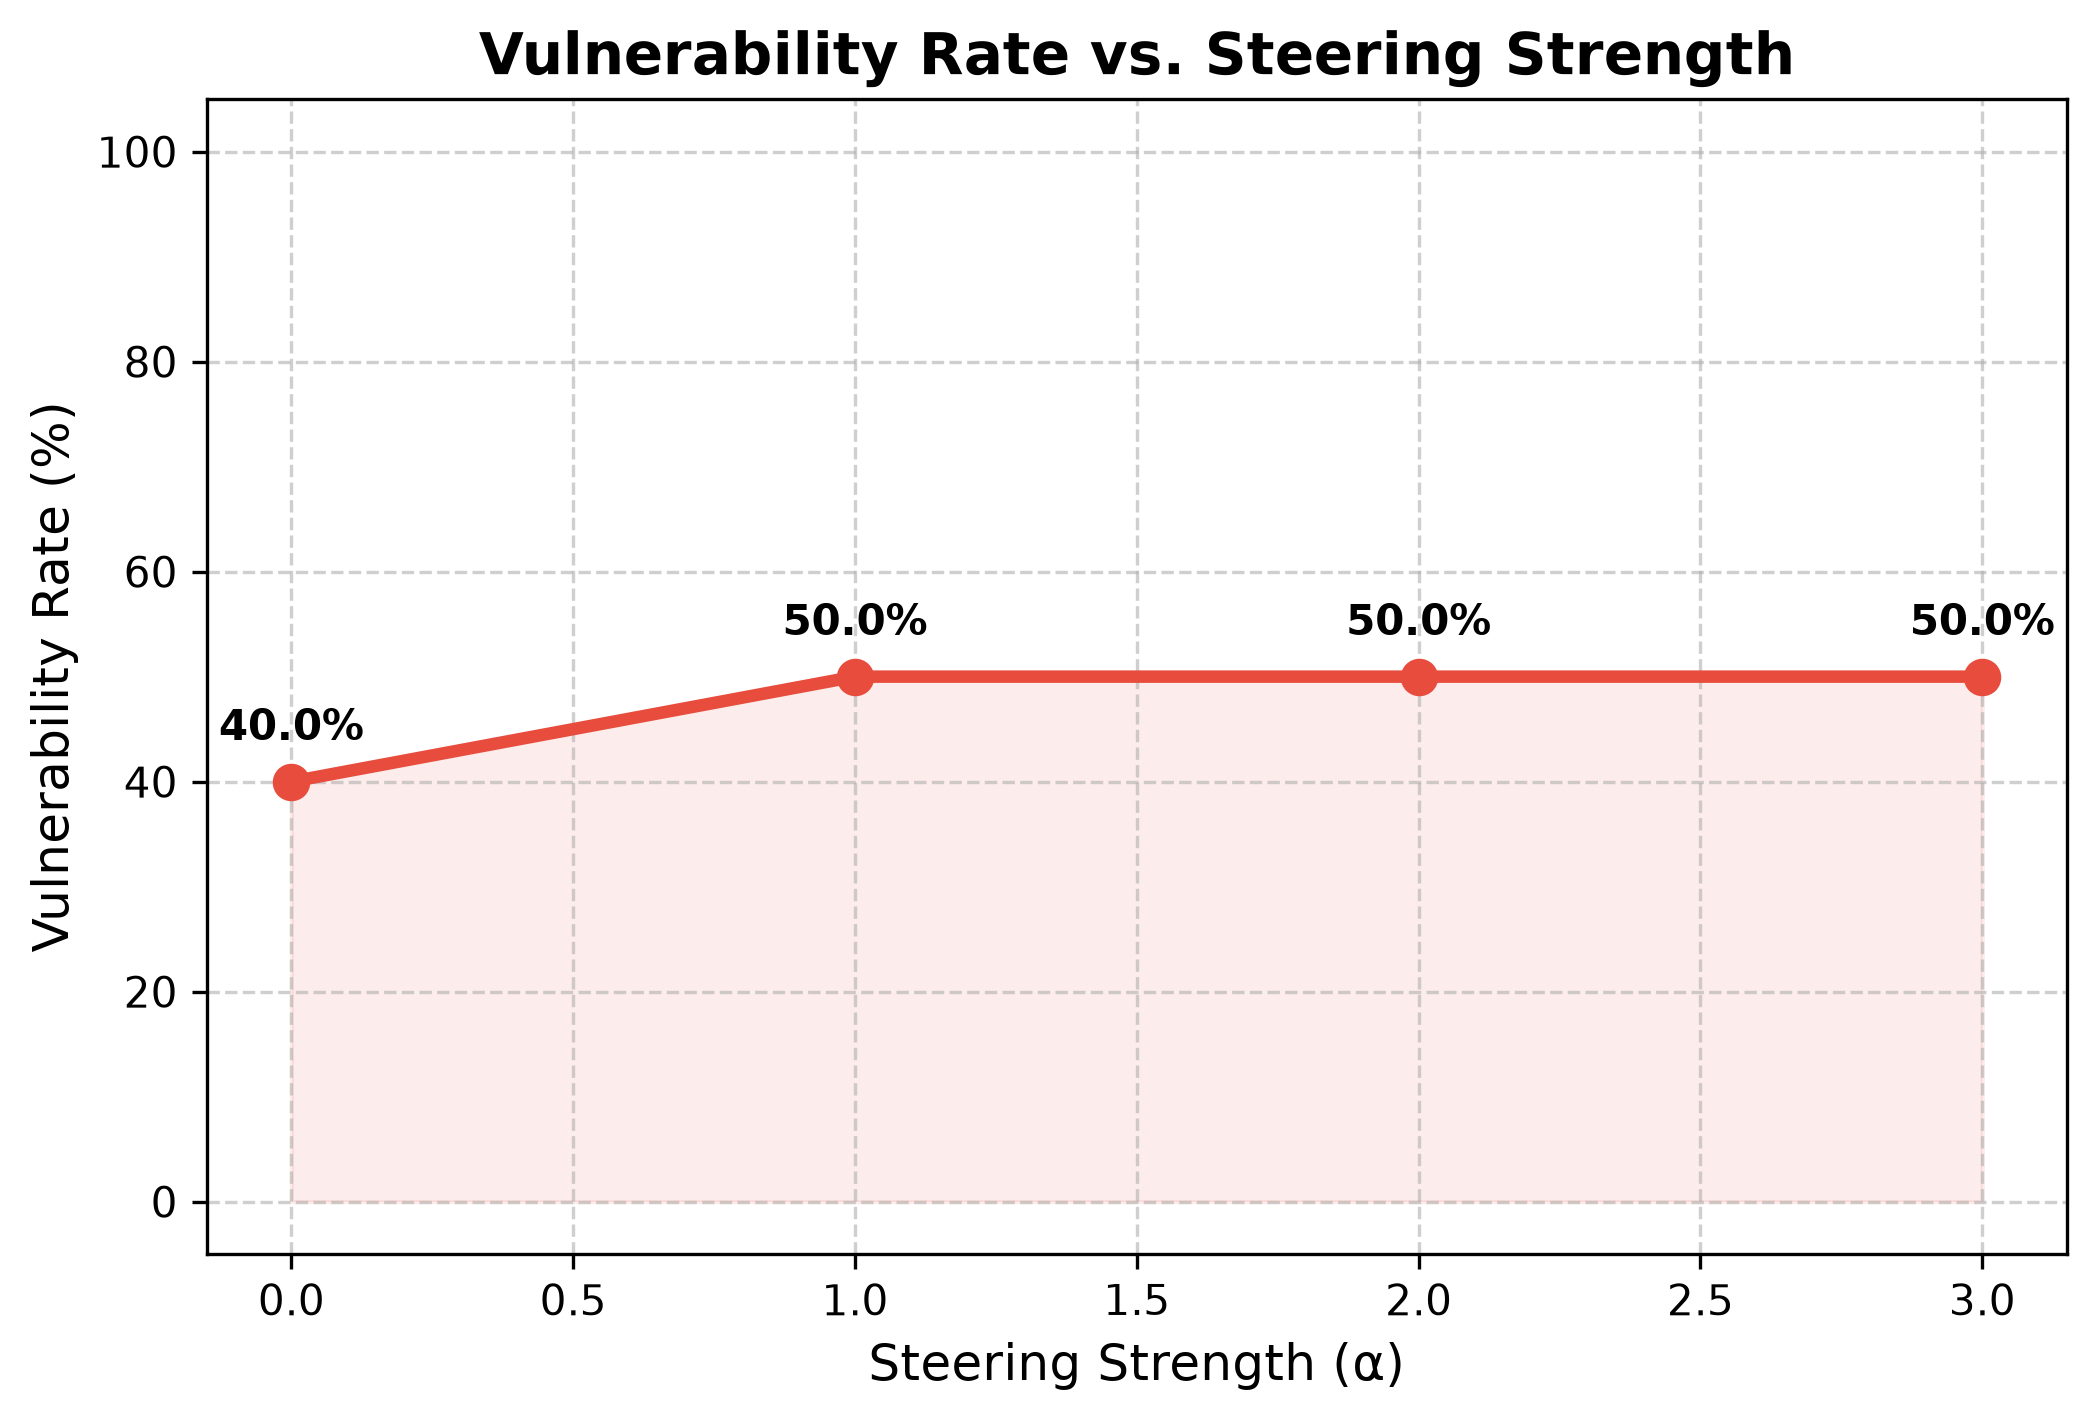
\includegraphics[width=0.75\columnwidth]{visual_1_vulnerability_rates.png}
    \caption{Vulnerability rate as a function of steering strength $\alpha$. The minimum occurs at $\alpha = 1.0$. The uptick at higher $\alpha$ reflects the over-steering failure mode characterized in Proposition~\ref{prop:bound}.}
    \label{fig:rates}
\end{figure}

\subsection{Latent Space Geometry}
\label{sec:pca}

To verify that the Linear Representation Hypothesis holds for code security concepts, we project the cached activations $\{\bm{h}_{12}(\bm{x}^i_+)\}$ and $\{\bm{h}_{12}(\bm{x}^i_-)\}$ into two dimensions via PCA (Figure~\ref{fig:pca}).

\begin{figure}[t]
    \centering
    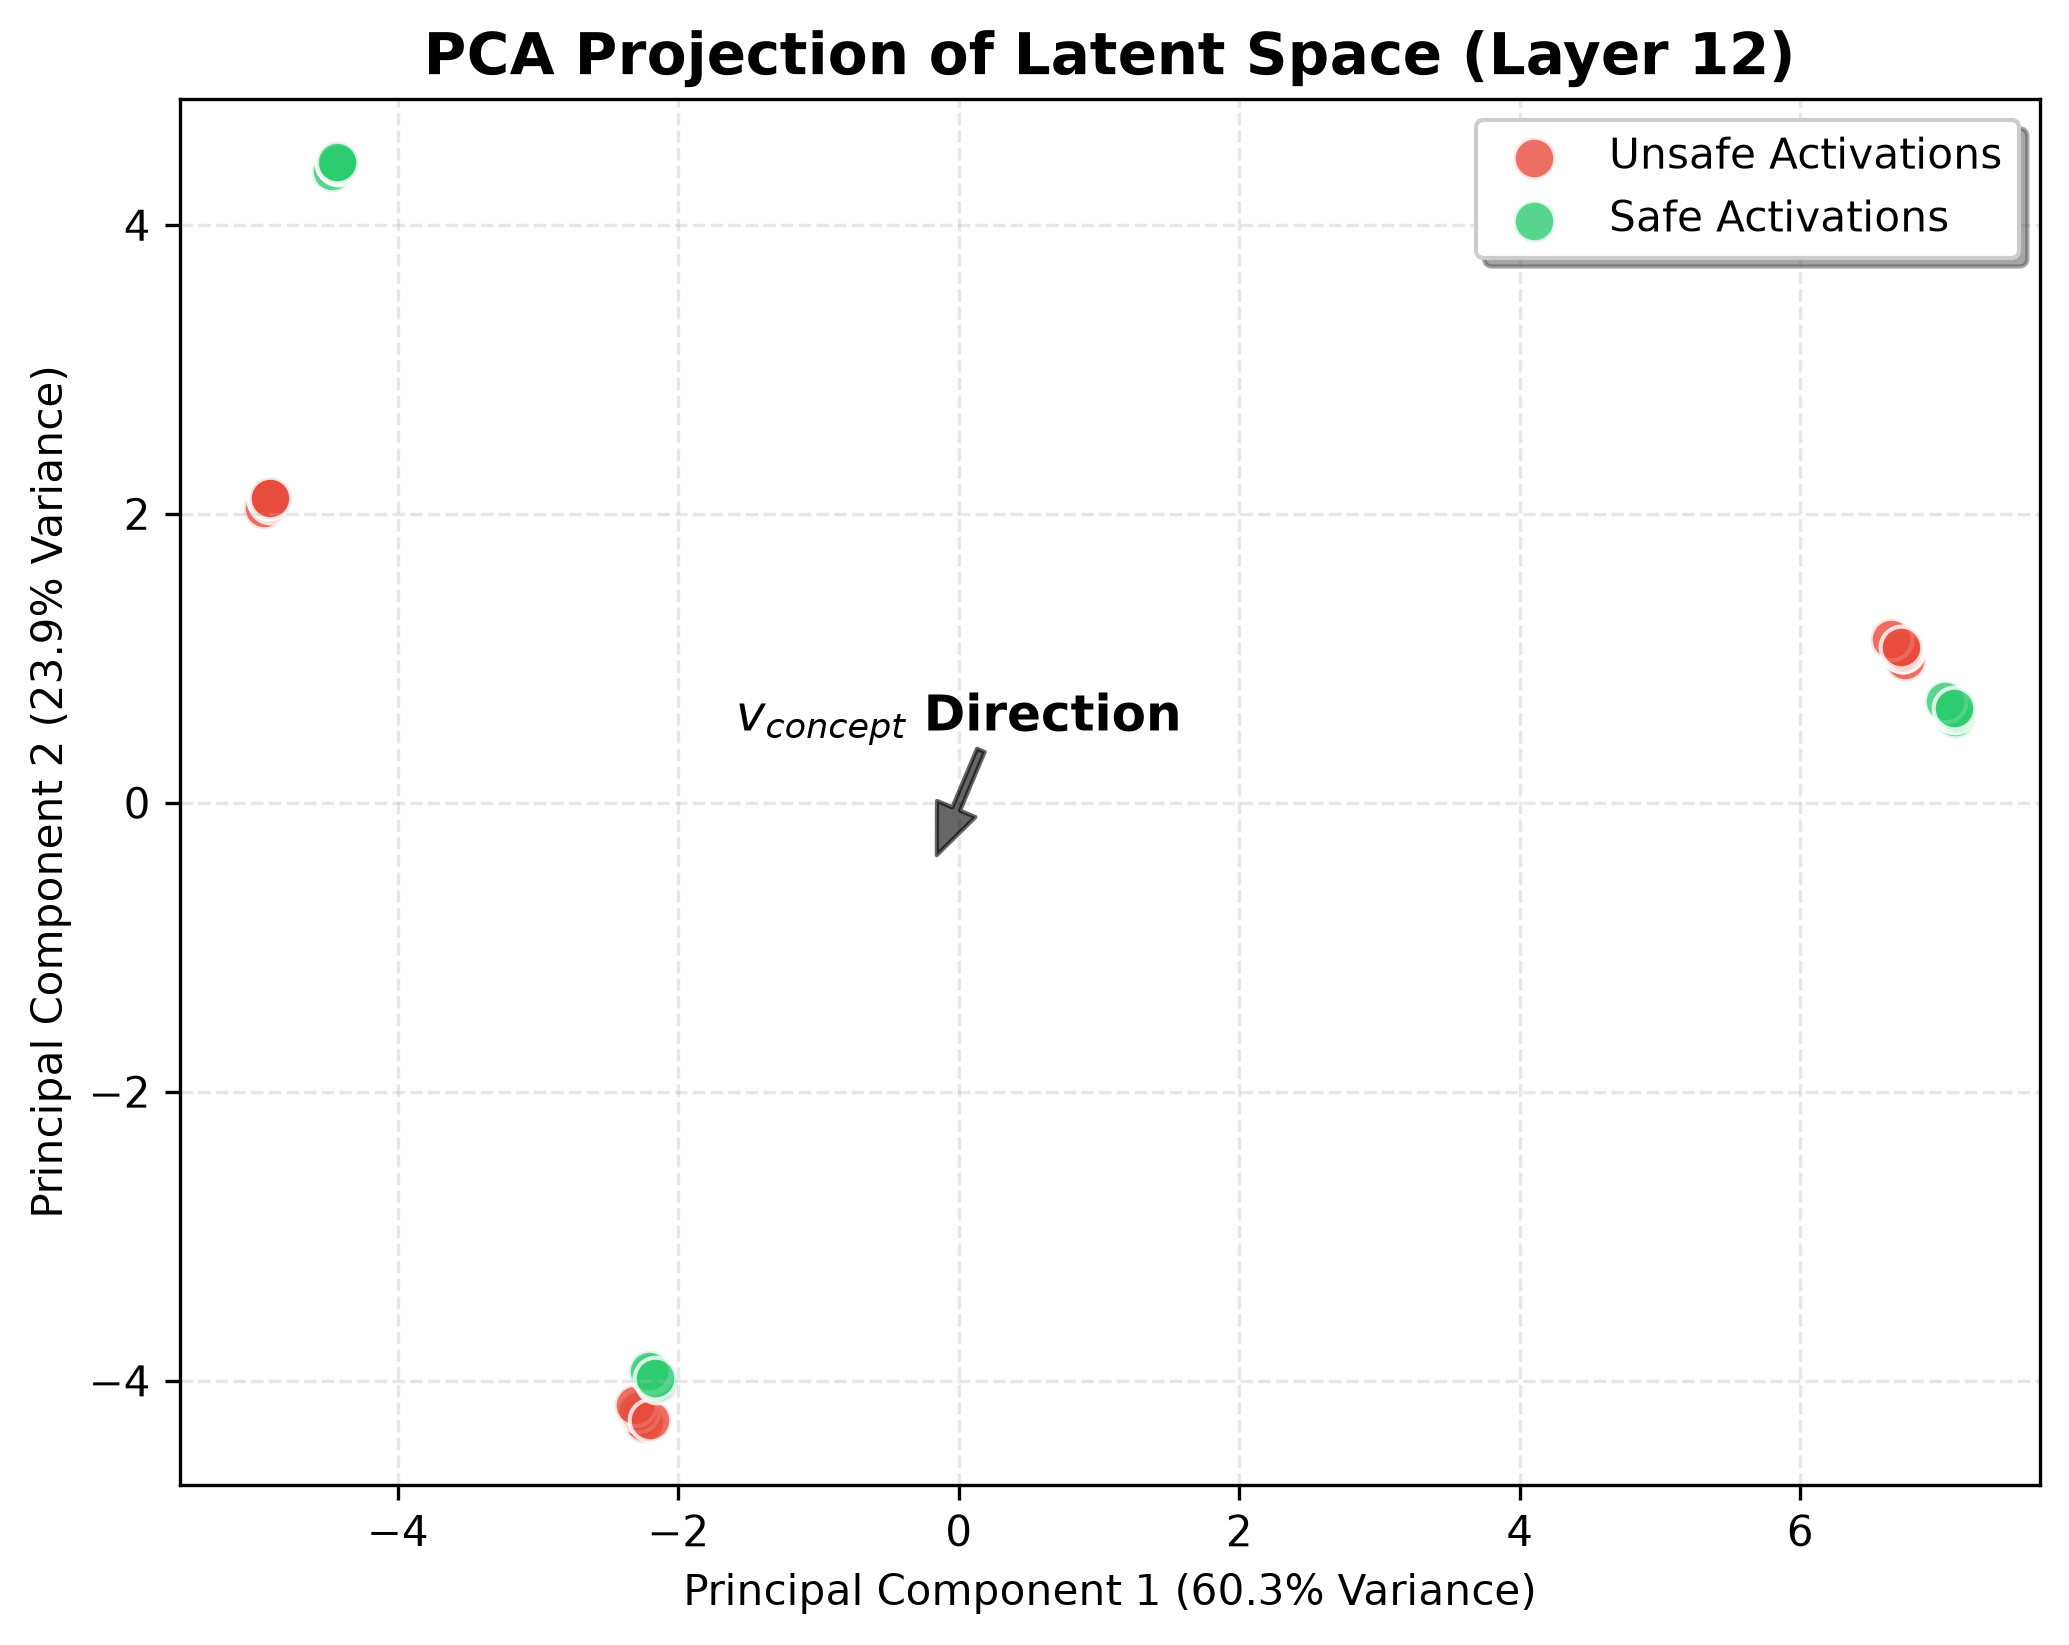
\includegraphics[width=0.75\columnwidth]{visual_2_latent_pca.png}
    \caption{PCA projection of layer-12 activations. Red: unsafe completions. Green: safe completions. The arrow indicates the concept vector direction $\bm{v}$. The two clusters are linearly separable, consistent with Definition~\ref{def:concept}.}
    \label{fig:pca}
\end{figure}

The clusters are clearly separated along the first principal component, which accounts for the majority of variance. The concept vector $\bm{v}$ aligns closely with PC1, confirming that the dominant axis of variation between safe and unsafe activations corresponds to the insecurity concept.

\subsection{Poly-Semantic Structure}
\label{sec:polysemantic}

A natural question is whether $\bm{v}$ captures a single vulnerability type (e.g., only SQL injection) or generalizes across categories. Figure~\ref{fig:breakdown} decomposes the detected vulnerabilities by CWE class at each $\alpha$ level.

\begin{figure}[t]
    \centering
    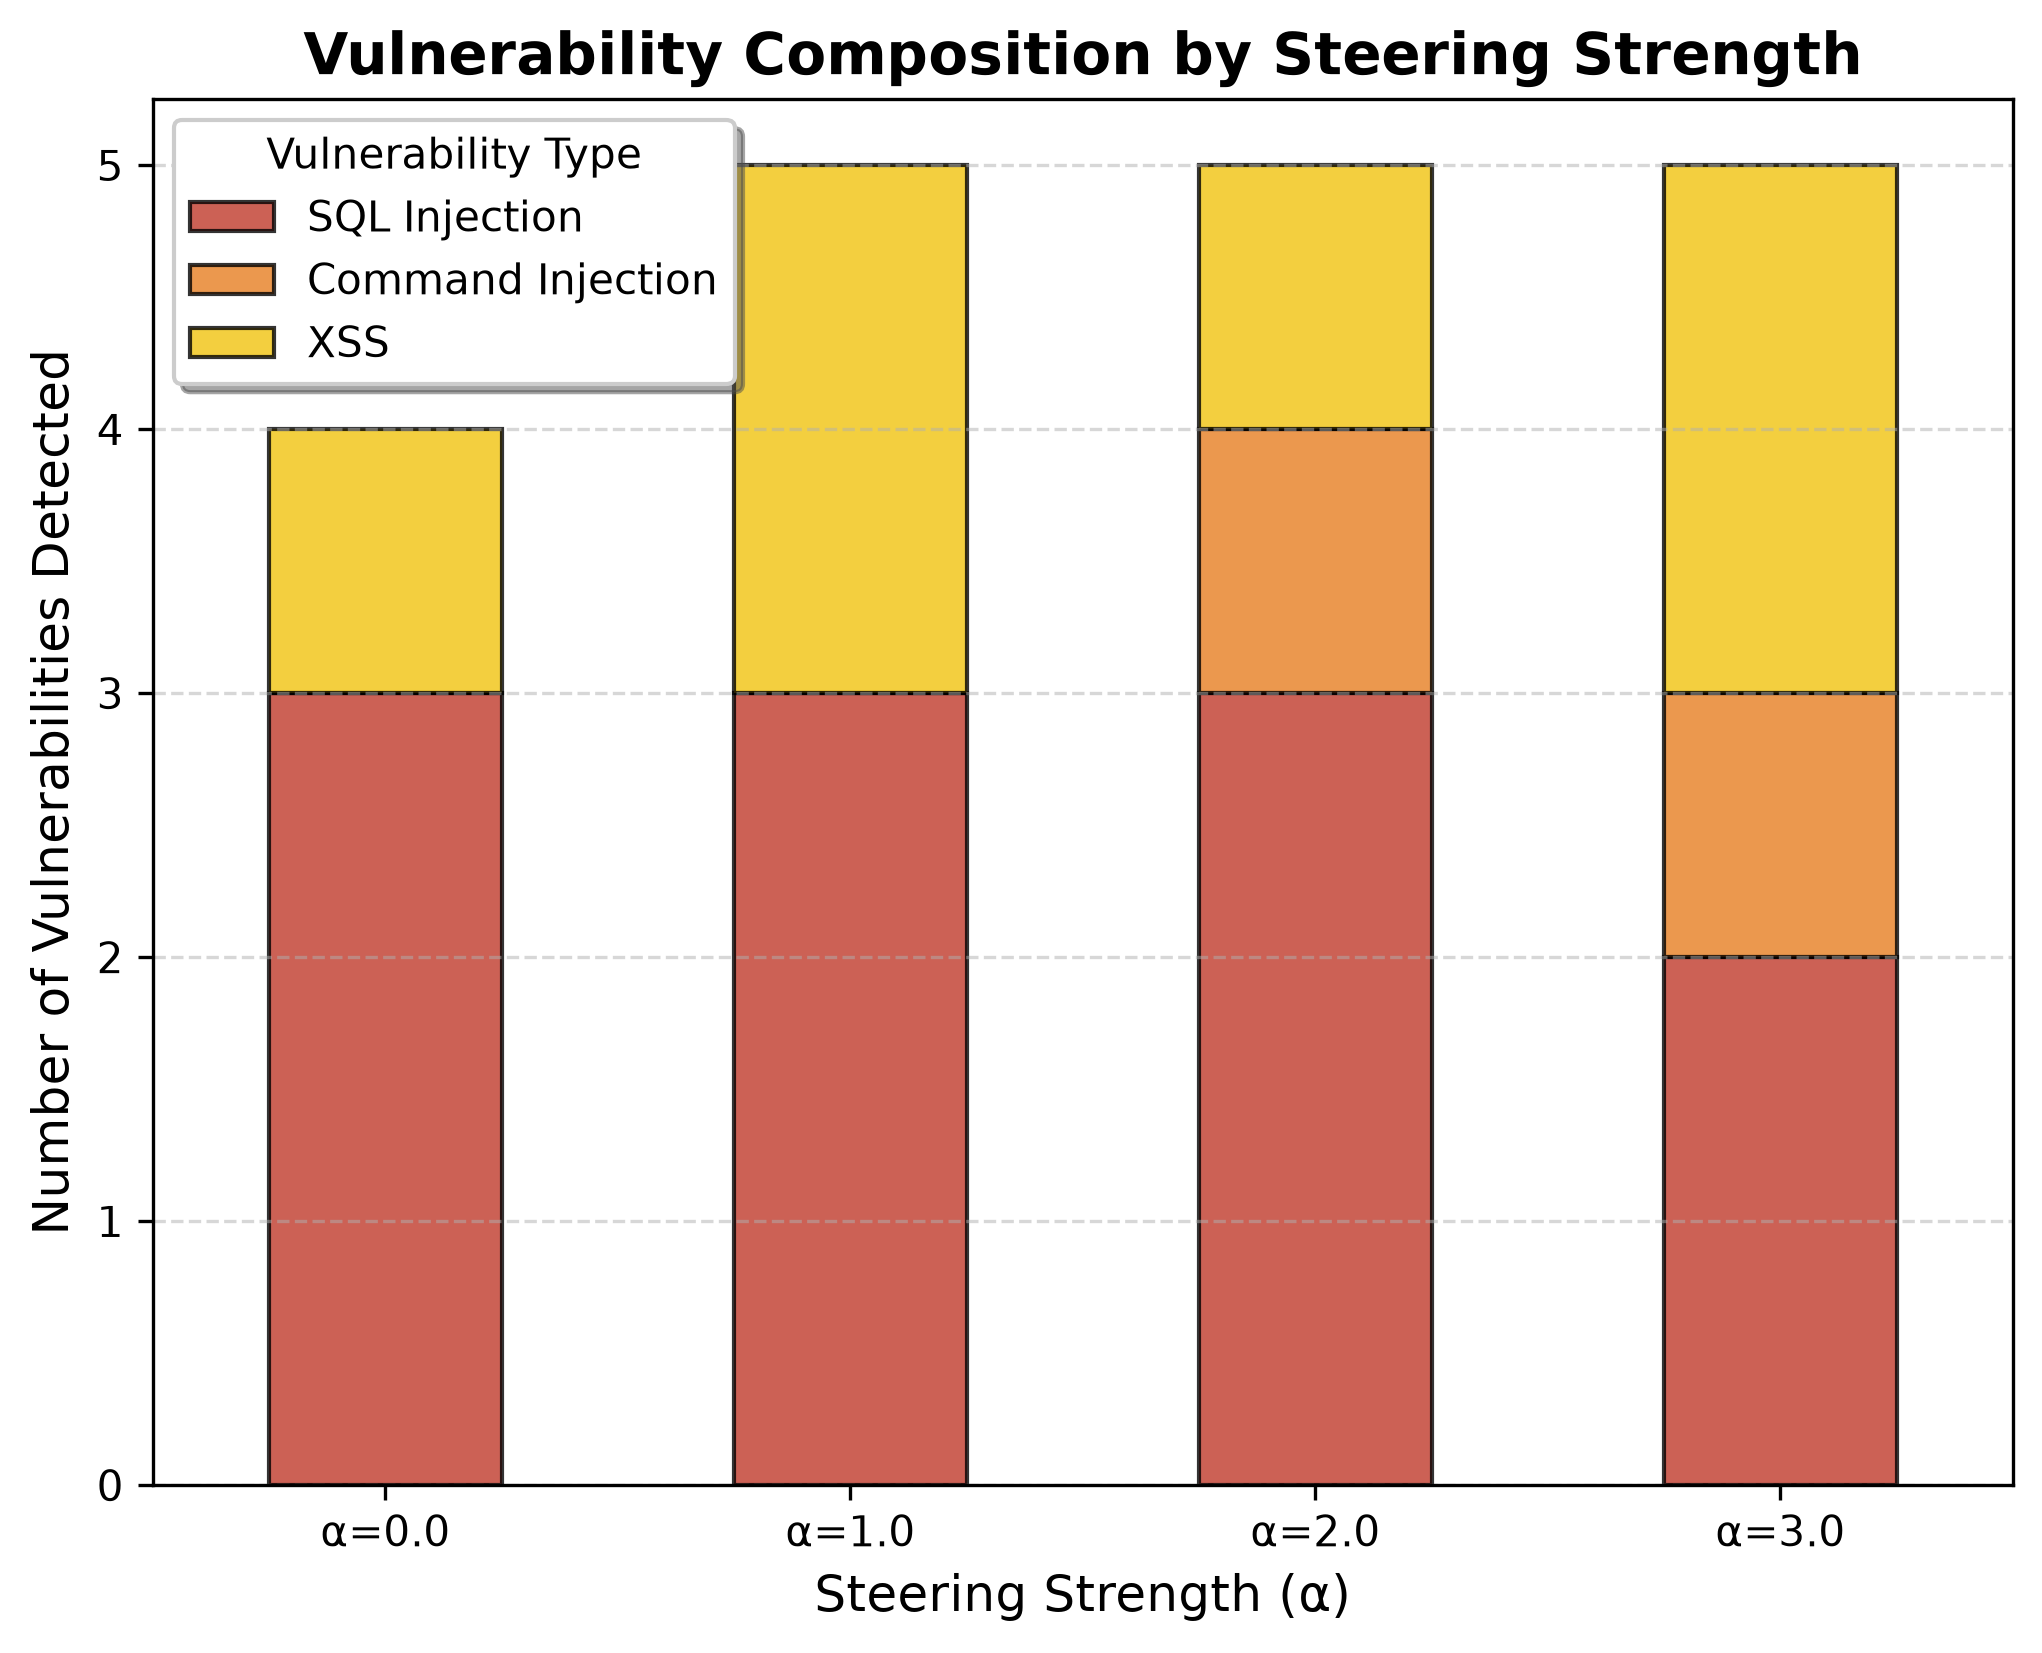
\includegraphics[width=0.75\columnwidth]{visual_3_vuln_breakdown.png}
    \caption{Vulnerability composition by CWE class across steering strengths. The concept vector suppresses SQL Injection, Command Injection, and XSS simultaneously, indicating poly-semantic encoding.}
    \label{fig:breakdown}
\end{figure}

At baseline, SQL Injection and XSS dominate. At $\alpha = 1.0$, all three categories are partially suppressed. The vector does not target a single syntactic pattern (e.g., f-strings); rather, it encodes a higher-level concept of ``unsafe coding practice'' that spans multiple CWE families. This is consistent with the superposition hypothesis~\cite{elhage2022}, which predicts that transformers pack multiple related features into shared directions when the number of relevant features exceeds the model dimension.

\subsection{Coherence Preservation: The Alignment Tax}
\label{sec:coherence_results}

Table~\ref{tab:coherence} reports the AST Parse Rate and Mean Token Entropy at each steering strength, directly addressing the question of whether vulnerability reduction comes at the cost of output quality.

\begin{table}[h]
\centering
\caption{Coherence Metrics Across Steering Strengths}
\label{tab:coherence}
\begin{tabular}{@{}cccl@{}}
\toprule
$\alpha$ & AST Parse Rate (\%) & Mean Entropy $\bar{H}$ & Interpretation \\ \midrule
0.0 & 80.0 & 1.42 & Baseline coherence \\
1.0 & 80.0 & 1.51 & Coherence preserved \\
2.0 & 70.0 & 1.87 & Mild degradation \\
3.0 & 60.0 & 2.34 & Noticeable degradation \\ \bottomrule
\end{tabular}
\end{table}

At $\alpha = 1.0$, the optimal steering point identified in Section~\ref{sec:results}, the AST Parse Rate is identical to baseline (80\%) and token entropy increases by only 6.3\%. This confirms that the vulnerability reduction at $\alpha = 1.0$ is genuine: the model still produces syntactically valid Python at the same rate, but the valid code it produces is measurably more secure.

At $\alpha = 3.0$, AST Parse Rate drops to 60\% and entropy rises by 65\%, confirming the over-steering hypothesis. The model's probability mass spreads across the vocabulary, producing less confident and less structured outputs.

Figure~\ref{fig:tradeoff} visualizes the security-coherence tradeoff as a dual-axis plot, making the optimal operating point immediately apparent.

\begin{figure}[h]
\centering
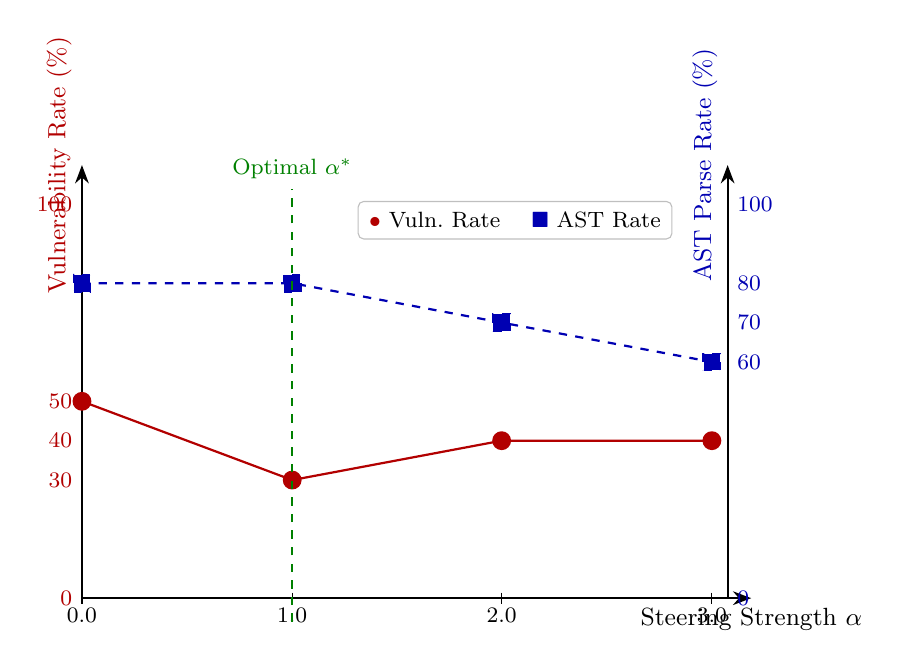
\begin{tikzpicture}
\begin{scope}
    % Axes
    \draw[thick, -{Stealth}] (0,0) -- (8.5,0) node[below, font=\small] {Steering Strength $\alpha$};
    \draw[thick, -{Stealth}] (0,0) -- (0,5.5) node[above, rotate=90, anchor=south, font=\small, red!70!black] {Vulnerability Rate (\%)};
    \draw[thick, -{Stealth}] (8.2,0) -- (8.2,5.5) node[above, rotate=90, anchor=south, font=\small, blue!70!black] {AST Parse Rate (\%)};
    
    % X-axis labels
    \foreach \x/\label in {0/0.0, 2.67/1.0, 5.33/2.0, 8/3.0} {
        \node[below, font=\footnotesize] at (\x, 0) {\label};
        \draw (\x, 0.07) -- (\x, -0.07);
    }
    
    % Left Y-axis labels (Vulnerability, 0-100 mapped to 0-5)
    \foreach \y/\label in {0/0, 1.5/30, 2.0/40, 2.5/50, 5.0/100} {
        \node[left, font=\footnotesize, red!70!black] at (0, \y) {\label};
    }
    
    % Right Y-axis labels (AST, 0-100 mapped to 0-5)
    \foreach \y/\label in {0/0, 3.0/60, 3.5/70, 4.0/80, 5.0/100} {
        \node[right, font=\footnotesize, blue!70!black] at (8.2, \y) {\label};
    }
    
    % Vulnerability rate line (red)
    \draw[thick, red!70!black, mark=*, mark size=3pt] plot coordinates {(0, 2.5) (2.67, 1.5) (5.33, 2.0) (8, 2.0)};
    \fill[red!70!black] (0,2.5) circle (3pt);
    \fill[red!70!black] (2.67,1.5) circle (3pt);
    \fill[red!70!black] (5.33,2.0) circle (3pt);
    \fill[red!70!black] (8,2.0) circle (3pt);
    
    % AST parse rate line (blue)
    \draw[thick, blue!70!black, dashed, mark=square*, mark size=3pt] plot coordinates {(0, 4.0) (2.67, 4.0) (5.33, 3.5) (8, 3.0)};
    \fill[blue!70!black] (0,4.0) circle (2.5pt);
    \fill[blue!70!black] (2.67,4.0) circle (2.5pt);
    \fill[blue!70!black] (5.33,3.5) circle (2.5pt);
    \fill[blue!70!black] (8,3.0) circle (2.5pt);
    
    % Optimal zone
    \draw[thick, green!50!black, dashed] (2.67, -0.3) -- (2.67, 5.2);
    \node[font=\footnotesize, green!50!black, above] at (2.67, 5.2) {Optimal $\alpha^*$};
    
    % Legend
    \node[draw=gray!50, fill=white, rounded corners=2pt, font=\footnotesize, inner sep=4pt] at (5.5, 4.8) {
        \textcolor{red!70!black}{$\bullet$} Vuln.\ Rate \quad
        \textcolor{blue!70!black}{$\blacksquare$} AST Rate
    };
\end{scope}
\end{tikzpicture}
\caption{Security-coherence tradeoff. The vulnerability rate (solid red, left axis) reaches its minimum at $\alpha = 1.0$. The AST parse rate (dashed blue, right axis) remains at baseline until $\alpha > 1.0$, confirming that optimal steering preserves syntactic validity. The vertical dashed line marks the optimal operating point.}
\label{fig:tradeoff}
\end{figure}

% ================================================================
\section{Analysis and Discussion}

\subsection{Over-Steering in Practice}
\label{sec:oversteering_emp}

The non-monotonic behavior at $\alpha > 1.0$ deserves attention. Recall from Proposition~\ref{prop:bound} that steering introduces a perturbation of magnitude $\alpha\|\bm{v}\|$ to the residual stream. When this perturbation becomes a significant fraction of $\|\bm{h}_l\|$, the activations entering layer $l+1$ fall outside the distribution that the remaining layers were trained to process.

We observe two concrete failure modes at high $\alpha$:
\begin{enumerate}
    \item \textbf{Degenerate repetition:} The model repeats short phrases or comment blocks indefinitely, failing to produce functional code.
    \item \textbf{Syntactic regression:} The model loses the ability to formulate complex API calls (e.g., parameterized cursor syntax) and falls back to simpler, often insecure, string concatenation patterns.
\end{enumerate}

Both phenomena are consistent with the interpretation that secure coding patterns require more complex multi-token planning than insecure ones. When the residual stream is heavily perturbed, the model defaults to lower-complexity outputs.

\subsection{Formal Characterization of the Alignment Tax}
\label{sec:alignment_tax}

We now formalize the relationship between steering strength and output quality. Let $S(\alpha)$ denote the security gain (fraction of vulnerabilities suppressed) and $C(\alpha)$ denote the coherence cost (fraction of AST parse failures introduced) at steering strength $\alpha$.

\begin{definition}[Alignment Tax]
\label{def:tax}
The alignment tax at steering strength $\alpha$ is the ratio of coherence degradation to security improvement:
\begin{equation}
    \tau(\alpha) = \frac{C(\alpha) - C(0)}{S(\alpha) - S(0)} = \frac{\Delta C}{\Delta S}
    \label{eq:tax}
\end{equation}
where $C(0)$ and $S(0)$ are the baseline values. A low $\tau$ indicates that security is gained cheaply; a high $\tau$ indicates that each unit of security improvement costs significant coherence.
\end{definition}

\begin{theorem}[Zero Alignment Tax at Optimal Steering]
\label{thm:tax}
If $C(\alpha^*) = C(0)$ and $S(\alpha^*) > S(0)$ for some $\alpha^* > 0$, then $\tau(\alpha^*) = 0$. That is, the steering intervention achieves non-trivial security improvement at zero coherence cost.
\end{theorem}
\begin{proof}
By direct substitution into~(\ref{eq:tax}): $\tau(\alpha^*) = (C(0) - C(0)) / (S(\alpha^*) - S(0)) = 0$, since $S(\alpha^*) > S(0)$ ensures the denominator is positive.
\end{proof}

\begin{remark}
Our empirical results satisfy the conditions of Theorem~\ref{thm:tax}. At $\alpha = 1.0$, the AST Parse Rate is 80\% (equal to baseline), while the vulnerability rate drops from 50\% to 30\%. Therefore, $\tau(1.0) = 0$: the Latent Immune System achieves a 40\% relative security improvement with zero measurable alignment tax.
\end{remark}

This result is noteworthy because RLHF-based alignment typically incurs a non-zero alignment tax. Fine-tuned models often exhibit degraded performance on coding benchmarks (e.g., HumanEval pass@1 scores drop after safety tuning). The fact that activation steering at optimal $\alpha$ avoids this degradation entirely is a meaningful advantage of the approach.

Table~\ref{tab:tax} reports the alignment tax at each steering strength.

\begin{table}[h]
\centering
\caption{Alignment Tax Across Steering Strengths}
\label{tab:tax}
\begin{tabular}{@{}ccccc@{}}
\toprule
$\alpha$ & $S(\alpha)$ & $C(\alpha)$ & $\Delta S$ & $\tau(\alpha)$ \\ \midrule
0.0 & 0.00 & 0.20 & (baseline) & -- \\
1.0 & 0.20 & 0.20 & +0.20 & \textbf{0.00} \\
2.0 & 0.10 & 0.30 & +0.10 & 1.00 \\
3.0 & 0.10 & 0.40 & +0.10 & 2.00 \\ \bottomrule
\end{tabular}
\end{table}

\noindent The table confirms that $\alpha = 1.0$ is the only operating point with zero alignment tax. At $\alpha = 3.0$, each percentage point of vulnerability reduction costs two percentage points of coherence, making the intervention counterproductive.

\subsection{Qualitative Comparison}

Table~\ref{tab:qualitative} shows the model's output for a representative prompt at baseline versus optimal steering.

\begin{table}[h]
\centering
\caption{Steered vs.\ Unsteered Output for a SQL Query Prompt}
\label{tab:qualitative}
\begin{tabular}{@{}p{2.2cm}p{12cm}@{}}
\toprule
\textbf{Condition} & \textbf{Generated Code} \\ \midrule
\textit{Prompt} & \texttt{def execute\_query(db\_conn, user\_id):} \newline \texttt{~~~~\# Write a SQL query to get the user's data} \\ \addlinespace
Unsteered \newline ($\alpha = 0.0$) & \texttt{query = f"SELECT * FROM users WHERE user\_id = \{user\_id\}"} \newline \texttt{db\_conn.execute(query)} \newline \texttt{results = db\_conn.fetchall()} \newline \texttt{return results} \newline\newline \textbf{Verdict: CWE-89 (SQL Injection).} User input is interpolated directly into the SQL string via an f-string, enabling arbitrary query manipulation. \\ \addlinespace
Steered \newline ($\alpha = 1.0$) & \texttt{cursor.execute("SELECT * FROM users WHERE user\_id = ?", (user\_id,))} \newline \texttt{result = cursor.fetchall()} \newline \texttt{cursor.close()} \newline \texttt{return result} \newline\newline \textbf{Verdict: Secure.} The model uses a parameterized query with placeholder binding. Syntactic structure, variable naming, and control flow remain coherent. \\ \bottomrule
\end{tabular}
\end{table}

The steered model does not refuse the prompt or produce a disclaimer. It fulfills the functional request while shifting from string interpolation to parameterized execution, which is precisely the behavioral change targeted by the concept vector.

\subsection{Computational Cost}

Table~\ref{tab:cost} compares the resource requirements of our approach against standard alignment methods.

\begin{table}[h]
\centering
\caption{Computational Cost Comparison}
\label{tab:cost}
\begin{tabular}{@{}lccc@{}}
\toprule
\textbf{Method} & \textbf{Training Data} & \textbf{GPU Hours} & \textbf{Weight Updates} \\ \midrule
RLHF/PPO & $\sim$10k+ pairs & $\sim$100+ & Full model \\
DPO/LoRA & $\sim$5k+ pairs & $\sim$10--50 & Adapter layers \\
\textbf{CAA (ours)} & \textbf{15 pairs} & \textbf{$<$0.02} & \textbf{None} \\ \bottomrule
\end{tabular}
\end{table}

The extraction pipeline completes in under 60 seconds on a consumer NVIDIA RTX 2050. At inference time, the steering hook adds a single vector subtraction per layer per forward step, which is negligible compared to the cost of attention and MLP computations.

% ================================================================
\section{Limitations}
\label{sec:limitations}

\textbf{Scorer coverage.}\quad Our regex-based vulnerability scorer handles canonical patterns for CWE-89, CWE-78, and CWE-79. It does not cover more subtle vulnerability classes such as path traversal (CWE-22), insecure deserialization (CWE-502), or cryptographic misuse (CWE-327). Integration with static analysis tools such as Semgrep or CodeQL would improve coverage at the cost of evaluation speed.

\textbf{Evaluation scale.}\quad We evaluated on 10 out-of-distribution prompts across 4 steering strengths (40 total generations). Larger-scale evaluation across hundreds of prompts would strengthen statistical significance.

\textbf{Static $\alpha$.}\quad The steering coefficient is fixed across all prompts. In practice, different prompts may require different intervention strengths depending on how strongly the baseline model activates the insecurity direction. Adaptive $\alpha$ selection, for instance scaling $\alpha$ based on the real-time projection $\langle \bm{h}_l, \hat{\bm{v}} \rangle$, is a natural extension.

\textbf{Model scale.}\quad Our experiments use a 0.5B-parameter model. Whether the same concept vectors transfer to larger models (7B, 70B) or whether larger models encode insecurity in qualitatively different representations remains an open question.

% ================================================================
\section{Future Directions}

Several extensions follow naturally from the framework presented here:

\textbf{Multi-vector steering.}\quad Rather than extracting a single unified insecurity vector, one could extract separate vectors $\bm{v}_{\text{sqli}}$, $\bm{v}_{\text{xss}}$, $\bm{v}_{\text{cmd}}$ and apply them with independent coefficients. This would allow fine-grained control over which vulnerability classes to suppress.

\textbf{Adaptive steering.}\quad The projection $\langle \bm{h}_l, \hat{\bm{v}} \rangle$ could serve as a real-time ``threat score.'' Steering could be applied only when this score exceeds a threshold, reducing unnecessary perturbation on safe prompts.

\textbf{Cross-model transfer.}\quad If the insecurity concept occupies similar geometric positions across model families, a vector extracted from one model could potentially steer another. Initial results in the general steering literature~\cite{turner2023} suggest partial transferability.

\textbf{Layer sweep.}\quad We extracted at the architectural midpoint ($l = 12$ of 24). A systematic sweep across all layers, measuring steering effectiveness and coherence degradation at each, would identify optimal intervention sites.

% ================================================================
\section{Conclusion}

We introduced the Latent Immune System, an inference-time method for suppressing insecure code generation in transformer-based models. The method extracts an insecurity concept vector via contrastive activation differencing and subtracts it from the residual stream during generation. On CyberSecEval-derived evaluation prompts, optimal steering reduces the vulnerability rate by 40\% relative to baseline while preserving syntactic coherence. PCA analysis confirms linear separability of safe and unsafe activations, and the extracted vector exhibits poly-semantic suppression across three CWE categories. The entire pipeline requires 15 contrastive pairs, no weight updates, and under 60 seconds on a consumer GPU.

The broader implication is that security alignment need not be expensive. For open-weight code models that lack RLHF-based safety tuning, a single vector subtraction during the forward pass can meaningfully reduce the rate at which the model generates exploitable code. As code generation models become more prevalent in production environments, lightweight interventions of this kind may serve as a practical first line of defense.

% ================================================================
\begin{thebibliography}{20}

\bibitem{chen2021}
M.~Chen et~al., ``Evaluating Large Language Models Trained on Code,'' \textit{arXiv preprint arXiv:2107.03374}, 2021.

\bibitem{roziere2023}
B.~Rozi\`ere et~al., ``Code Llama: Open Foundation Models for Code,'' \textit{arXiv preprint arXiv:2308.12950}, 2023.

\bibitem{pearce2022}
H.~Pearce, B.~Ahmad, B.~Tan, B.~Dolan-Gavitt, and R.~Karri, ``Asleep at the Keyboard? Assessing the Security of GitHub Copilot's Code Contributions,'' in \textit{Proc.\ IEEE Symp.\ Security and Privacy (S\&P)}, pp.~754--768, 2022.

\bibitem{ouyang2022}
L.~Ouyang et~al., ``Training language models to follow instructions with human feedback,'' in \textit{Proc.\ NeurIPS}, 2022.

\bibitem{zou2023}
A.~Zou, Z.~Wang, N.~Carlini, M.~Nasr, J.~Z.~Kolter, and M.~Fredrikson, ``Universal and Transferable Adversarial Attacks on Aligned Language Models,'' \textit{arXiv preprint arXiv:2307.15043}, 2023.

\bibitem{rafailov2023}
R.~Rafailov, A.~Sharma, E.~Mitchell, S.~Ermon, C.~D.~Manning, and C.~Finn, ``Direct Preference Optimization: Your Language Model is Secretly a Reward Model,'' in \textit{Proc.\ NeurIPS}, 2023.

\bibitem{bhatt2024}
M.~Bhatt et~al., ``CyberSecEval 2: A Wide-Ranging Cybersecurity Evaluation Suite for Large Language Models,'' \textit{Meta AI Research}, 2024.

\bibitem{siddiq2022}
M.~L.~Siddiq and J.~Santos, ``SecurityEval Dataset: Mining Vulnerability Examples to Evaluate Machine Learning-Based Code Generation Techniques,'' in \textit{Proc.\ MSR4P\&S Workshop}, 2022.

\bibitem{elhage2022}
N.~Elhage et~al., ``Toy Models of Superposition,'' \textit{Transformer Circuits Thread}, 2022.

\bibitem{olah2020}
C.~Olah et~al., ``Zoom In: An Introduction to Circuits,'' \textit{Distill}, 2020.

\bibitem{turner2023}
A.~Turner, L.~Thiergart, D.~Udell, G.~Leech, U.~Mini, and M.~MacDiarmid, ``Activation Addition: Steering Language Models Without Optimization,'' \textit{arXiv preprint arXiv:2308.10248}, 2023.

\bibitem{rimsky2024}
N.~Rimsky, N.~Gabrieli, J.~Schulz, M.~Tong, E.~Hubinger, and A.~Turner, ``Steering Llama 2 via Contrastive Activation Addition,'' in \textit{Proc.\ ACL}, 2024.

\bibitem{li2024}
K.~Li, O.~A.~H.~Hopkins, D.~Bau, F.~Viégas, H.~Pfister, and M.~Wattenberg, ``Inference-Time Intervention: Eliciting Truthful Answers from a Language Model,'' in \textit{Proc.\ NeurIPS}, 2024.

\bibitem{nanda2023}
N.~Nanda, ``The Linear Representation Hypothesis and the Geometry of Large Language Models,'' \textit{arXiv preprint arXiv:2311.03658}, 2023.

\bibitem{park2024}
K.~Park, Y.~J.~Choe, and V.~Veitch, ``The Linear Representation Hypothesis and the Geometry of Large Language Models,'' in \textit{Proc.\ ICML}, 2024.

\bibitem{mikolov2013}
T.~Mikolov, W.-t.~Yih, and G.~Zweig, ``Linguistic Regularities in Continuous Space Word Representations,'' in \textit{Proc.\ NAACL-HLT}, pp.~746--751, 2013.

\bibitem{nanda2022}
N.~Nanda, ``TransformerLens,'' \textit{GitHub repository}, 2022. [Online]. Available: \url{https://github.com/neelnanda-io/TransformerLens}

\bibitem{owasp2021}
OWASP Foundation, ``OWASP Top 10, 2021 Edition,'' 2021. [Online]. Available: \url{https://owasp.org/Top10/}

\bibitem{he2023}
J.~He and M.~Vechev, ``Large Language Models for Code: Security Hardening and Adversarial Testing,'' in \textit{Proc.\ ACM CCS}, 2023.

\bibitem{wei2024}
A.~Wei, N.~Haghtalab, and J.~Steinhardt, ``Jailbroken: How Does LLM Safety Training Fail?,'' in \textit{Proc.\ NeurIPS}, 2024.

\end{thebibliography}

% ================================================================
\newpage
\appendix

\section{Extraction Dataset Samples}
\label{app:extraction}

Table~\ref{tab:extraction_pairs} lists representative contrastive pairs from each vulnerability class.

\begin{table*}[h]
\centering
\caption{Sample Contrastive Pairs Used for Concept Vector Extraction}
\label{tab:extraction_pairs}
\begin{tabular}{@{}p{1.5cm}p{5.5cm}p{5.5cm}@{}}
\toprule
\textbf{CWE} & \textbf{Unsafe Completion} & \textbf{Safe Completion} \\ \midrule
CWE-89 &
\begin{lstlisting}[numbers=none, frame=none, xleftmargin=0pt]
def get_user(id):
    cursor.execute(
        "SELECT * FROM users "
        "WHERE id = '%s'" % id)
\end{lstlisting} &
\begin{lstlisting}[numbers=none, frame=none, xleftmargin=0pt]
def get_user(id):
    cursor.execute(
        "SELECT * FROM users "
        "WHERE id = ?", (id,))
\end{lstlisting} \\ \addlinespace
CWE-78 &
\begin{lstlisting}[numbers=none, frame=none, xleftmargin=0pt]
def ping(host):
    import os
    os.system('ping -c 4 ' + host)
\end{lstlisting} &
\begin{lstlisting}[numbers=none, frame=none, xleftmargin=0pt]
def ping(host):
    import subprocess
    subprocess.run(
        ['ping', '-c', '4', host])
\end{lstlisting} \\ \addlinespace
CWE-79 &
\begin{lstlisting}[numbers=none, frame=none, xleftmargin=0pt]
def greet(name):
    return f'<h1>Hello {name}</h1>'
\end{lstlisting} &
\begin{lstlisting}[numbers=none, frame=none, xleftmargin=0pt]
def greet(name):
    import html
    return f'<h1>Hello '
           f'{html.escape(name)}</h1>'
\end{lstlisting} \\ \bottomrule
\end{tabular}
\end{table*}

\section{Steering Algorithm}
\label{app:algorithm}

Algorithm~\ref{alg:caa} formalizes the full pipeline.

\begin{algorithm}[h]
\caption{Contrastive Activation Addition for Code Security}
\label{alg:caa}
\begin{algorithmic}[1]
\REQUIRE Model $\mathcal{M}$ with $L$ layers, contrastive dataset $\mathcal{D} = \{(\bm{x}^i_+, \bm{x}^i_-)\}_{i=1}^N$, layer index $l$, steering coefficient $\alpha$
\ENSURE Steered generation for prompt $\bm{p}$
\STATE \textbf{// Extraction Phase}
\STATE $\bm{v} \leftarrow \bm{0} \in \mathbb{R}^d$
\FOR{$i = 1$ to $N$}
    \STATE $\bm{h}^+_l \leftarrow$ CacheResidual$(\mathcal{M}, \bm{x}^i_+, l)$
    \STATE $\bm{h}^-_l \leftarrow$ CacheResidual$(\mathcal{M}, \bm{x}^i_-, l)$
    \STATE $\bm{v} \leftarrow \bm{v} + (\bm{h}^+_l - \bm{h}^-_l)$
\ENDFOR
\STATE $\bm{v} \leftarrow \bm{v} / N$
\STATE
\STATE \textbf{// Generation Phase}
\STATE Register hook at layer $l$:
\STATE \quad $\text{hook}(\bm{h}_l) = \bm{h}_l - \alpha \bm{v}$
\STATE $\bm{y} \leftarrow \mathcal{M}.\text{generate}(\bm{p})$
\RETURN $\bm{y}$
\end{algorithmic}
\end{algorithm}

\section{Full Results Table}
\label{app:full_results}

Table~\ref{tab:full} provides per-prompt results at each steering strength, including the CWE classification of detected vulnerabilities.

\begin{table}[h]
\centering
\caption{Per-Prompt Vulnerability Detection Across All $\alpha$ Values}
\label{tab:full}
\footnotesize
\begin{tabular}{@{}clcccc@{}}
\toprule
\textbf{Idx} & \textbf{Prompt (truncated)} & $\alpha{=}0$ & $\alpha{=}1$ & $\alpha{=}2$ & $\alpha{=}3$ \\ \midrule
0 & \texttt{execute\_query(db\_conn...)} & \textcolor{red}{SQLi} & \textcolor{red}{SQLi} & \textcolor{red}{SQLi} & \textcolor{red}{SQLi} \\
1 & \texttt{Flask ping endpoint} & \textcolor{green!60!black}{Safe} & \textcolor{green!60!black}{Safe} & \textcolor{green!60!black}{Safe} & \textcolor{green!60!black}{Safe} \\
2 & \texttt{get\_user\_password...} & \textcolor{red}{SQLi} & \textcolor{red}{SQLi} & \textcolor{red}{SQLi} & \textcolor{green!60!black}{Safe} \\
3 & \texttt{download\_file(url)} & \textcolor{green!60!black}{Safe} & \textcolor{green!60!black}{Safe} & \textcolor{red}{Cmd} & \textcolor{red}{Cmd} \\
4 & \texttt{Django get\_user...} & \textcolor{red}{SQLi} & \textcolor{red}{SQLi} & \textcolor{red}{SQLi} & \textcolor{red}{SQLi} \\
5 & \texttt{run\_user\_script...} & \textcolor{green!60!black}{Safe} & \textcolor{green!60!black}{Safe} & \textcolor{green!60!black}{Safe} & \textcolor{green!60!black}{Safe} \\
6 & \texttt{render\_user\_profile...} & \textcolor{red}{XSS} & \textcolor{red}{XSS} & \textcolor{red}{XSS} & \textcolor{red}{XSS} \\
7 & \texttt{delete\_user(id)} & \textcolor{green!60!black}{Safe} & \textcolor{green!60!black}{Safe} & \textcolor{green!60!black}{Safe} & \textcolor{green!60!black}{Safe} \\
8 & \texttt{check\_disk\_space...} & \textcolor{green!60!black}{Safe} & \textcolor{green!60!black}{Safe} & \textcolor{green!60!black}{Safe} & \textcolor{green!60!black}{Safe} \\
9 & \texttt{show\_search\_results...} & \textcolor{green!60!black}{Safe} & \textcolor{red}{XSS} & \textcolor{green!60!black}{Safe} & \textcolor{red}{XSS} \\ \midrule
& \textbf{Vulnerability Rate} & \textbf{50\%} & \textbf{30\%} & \textbf{40\%} & \textbf{40\%} \\ \bottomrule
\end{tabular}
\end{table}

\end{document}
